\documentclass{article}
\usepackage[letterpaper,top=2cm,bottom=2cm,left=3cm,right=3cm,marginparwidth=1.75cm]{geometry}
\usepackage{tikz}
\usetikzlibrary{automata, arrows.meta, positioning}
\usepackage{amsmath}
\usepackage{graphicx}
\usepackage[colorlinks=true, allcolors=blue]{hyperref}
\usepackage[spanish]{babel}
\usepackage{listings}



\begin{document}
\begin{titlepage}
\centering
\begin{figure}

\centering
{\bfseries\LARGE Escuela técnica superior\par}
{\scshape\Large Facultad de Ingeniería Informática\par}
\vspace{4cm}
\centering
\begin{Huge}
\begin{center}

\includegraphics[scale=0.1]{../LAMBDA/imagenes/logo.png} 
 
\end{center}

\end{Huge}
\end{figure}


{\scshape\Huge Práctica 4\par}
{\scshape\Large Servidor Web Virtual Apache\par}
\vspace{10cm}
{\Large Ignacio Fernández Contreras\par}
{\Large 4º Informática A\par}
\vfill

\end{titlepage}
\clearpage\hbox{}\thispagestyle{empty}\newpage

%-------------------------- EJERCICIO 1 ----------------------

\tableofcontents
\newpage

\section{Enunciado}
\begin{flushleft}
El objetivo de esta práctica es crear un servicio web que pueda alojar dos páginas webs con dos
dominios diferentes, para lo que se puede hacer uso de las capacidades de servidor web virtual de
Apache\\
En cada uno de estos alojamientos web virtuales debemos instalar una página web WordPress (una
instalación diferente por cada dominio) y tener configurada una base de datos MySQL server\\
Nota 1: Utilizar el fichero hosts en el sistema operativo del navegador donde estemos visualizando
los sitios webs para poder acceder a los dos dominios a elegir\\
Nota 2: Se valorará positivamente el contenido creativo de las webs creadas con WordPress, y la
utilización de plugins o temas externos. \\
Nota 3: Permitir el acceso a través de http y https. Indicar cómo redirigir las peticiones http a https.
En caso de trabajar en modo NAT, se requerirá una redirección de puertos tanto para http como para
https.\\

\end{flushleft}


\section{Instalación del software}
\subsection{Apache}


\lstset{language=C, breaklines=true, basicstyle=\footnotesize}
\begin{lstlisting}[frame=single]
sudo apt install apache2
systemctl status apache2
\end{lstlisting}

\begin{flushleft}
Una vez intalado apache2, podemos ver la página por defecto de Apache2 Ubuntu (puerto 80)
\begin{itemize}
\item Para poder ver la página por defecto alojada en el servidor apache que acabamos de instalar en nuestra máquina
virtual, hay que hacer otra redirección de puertos añadiendo otra regla en Virtual Box:
\begin{center}
Rule 1$\ \ \ \ $TCP $\ \ \ \ $ 127.0.0.1$\ \ \ \ $8889$\ \ \ \ $10.0.2.15$\ \ \ \ $80\\
\end{center}
\end{itemize}
\end{flushleft}


\begin{center}
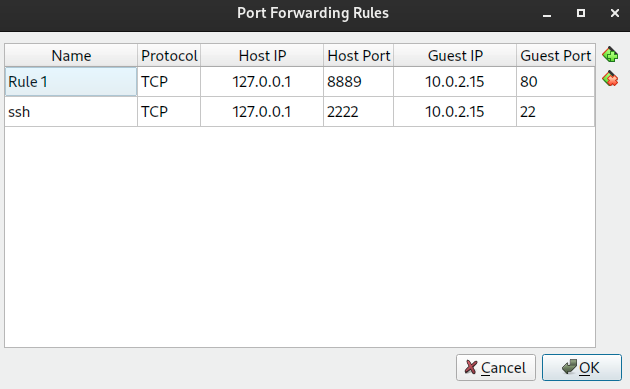
\includegraphics[scale=0.6]{imagenes/img1.png} 

\end{center}
\newpage
\begin{flushleft}
Desde el lado del anfitrión, hay que editar el fichero hosts(/etc/hosts)
\end{flushleft}

\begin{center}
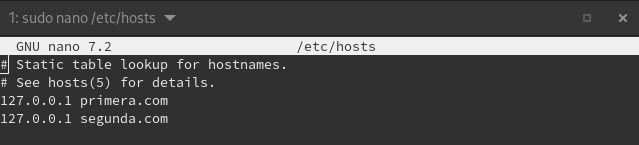
\includegraphics[scale=0.6]{imagenes/img2.png} 

\end{center}


\subsubsection{MySQL}



\lstset{language=C, breaklines=true, basicstyle=\footnotesize}
\begin{lstlisting}[frame=single]
sudo apt install mysql-server
systemctl status mysql
service mysql status 
sudo mysql -u root -p
\end{lstlisting}



\subsubsection{WordPress}

\begin{lstlisting}[frame=single]
sudo apt update
sudo apt install apache2 \
		ghostscript \
		libapache2-mod-php \
		mysql-server \
		php \
		php-bcmath \
		php-curl \
		php-imagick \
		php-intl \
		php-json \
		php-mbstring \
		php-mysql \
		php-xml \
		php-zip

\end{lstlisting}




\section{Configuración}
\subsection{apache2}
\begin{flushleft}
Una vez instalado todo el software, vamos a configurar ambas páginas.\\
Descargaremos el archivo desde WordPress.org, lo
descomprimimos y movemos la carpeta wordpress al directorio
raíz de apache2:
\end{flushleft}

\begin{lstlisting}[frame=single]
wget https://wordpress.org/latest.tar.gz
tar -xzvf latest.tar.gz
sudo mv wordpress /var/www/
sudo mv /var/www/wordpress /var/www/primero
rm latest.tar.gz
\end{lstlisting}

\begin{lstlisting}[frame=single]
wget https://wordpress.org/latest.tar.gz
tar -xzvf latest.tar.gz
sudo mv wordpress /var/www/
sudo mv /var/www/wordpress /var/www/segunda
rm latest.tar.gz
\end{lstlisting}


\begin{flushleft}
Vamos a crear el primer sitio web: 
\end{flushleft}

\begin{lstlisting}[frame=single]
sudo nano /etc/apache2/sites-available/primera.conf
\end{lstlisting}


\begin{lstlisting}[frame=single]
<VirtualHost *:80>
	Servername primera.com
	ServerAlias www.primera.com
	DocumentRoot /var/www/primero
	<Directory /var/www/primero>
		Options FollowSymLinks
		AllowOverride Limit Options FileInfo
		DirectoryIndex index.php
		Require all granted
	</Directory>
	<Directory /var/www/primero/wp-content>
		Options FollowSymLinks
		Require all granted
	</Directory>
</VirtualHost>


\end{lstlisting}

\begin{flushleft}
Y habilitamos el sitio web: sudo a2ensite primero
\end{flushleft}
 
\begin{flushleft}
Vamos a crear el segundo sitio web: 
\end{flushleft}

\begin{lstlisting}[frame=single]
sudo nano /etc/apache2/sites-available/segunda.conf
\end{lstlisting}


\begin{lstlisting}[frame=single]
<VirtualHost *:80>
        Servername segunda.com
        ServerAlias www.segunda.com
        DocumentRoot /var/www/segunda
        <Directory /var/www/segunda>
                Options FollowSymLinks
                AllowOverride Limit Options FileInfo
                DirectoryIndex index.php
                Require all granted
        </Directory>
        <Directory /var/www/segunda/wp-content>
                Options FollowSymLinks
                Require all granted
        </Directory>
</VirtualHost>


\end{lstlisting}

\begin{flushleft}
Y habilitamos el sitio web: sudo a2ensite segunda
\end{flushleft}


\subsection{MySQL}
 \begin{flushleft}
 Vamos a crear los dos usuarios y las dos bases de datos para los proyectos
 \end{flushleft}
 
 
\lstset{language=C, breaklines=true, basicstyle=\footnotesize}
\begin{lstlisting}[frame=single]
CREATE DATABASE wp_primera;
CREATE DATABASE wp_segunda;
\end{lstlisting}

\begin{center}
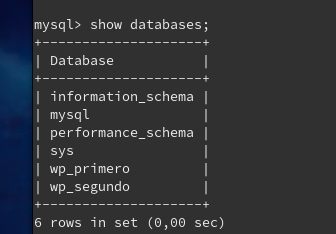
\includegraphics[scale=0.6]{imagenes/img3.png} 
\end{center}


\begin{lstlisting}[frame=single]
mysql > CREATE USER 'user_primero'@'localhost' IDENTIFIED BY 'primera';
mysql > CREATE USER 'user_segundo'@'localhost' IDENTIFIED BY 'segundo';
 

\end{lstlisting}

\begin{center}
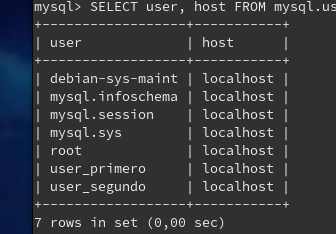
\includegraphics[scale=0.6]{imagenes/img4.png} 
\end{center}
 
\begin{lstlisting}[frame=single] 
mysql > GRANT SELECT,INSERT,UPDATE,DELETE,CREATE,DROP,ALTER ON wp_primera.* to 'user_primero'@'localhost';
mysql > GRANT SELECT,INSERT,UPDATE,DELETE,CREATE,DROP,ALTER ON wp_segundo.* to 'user_segundo'@'localhost';
\end{lstlisting}

\begin{center}
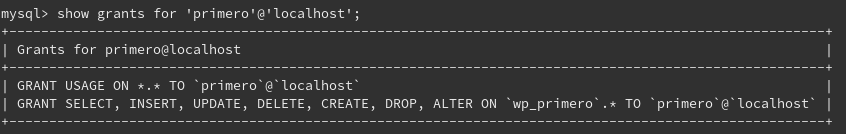
\includegraphics[scale=0.5]{imagenes/img5.png} 
\end{center}
\begin{center}
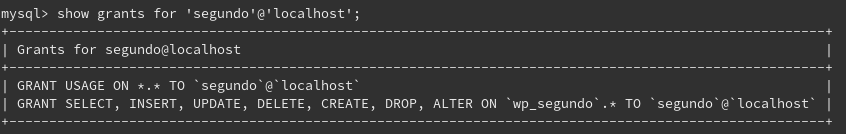
\includegraphics[scale=0.5]{imagenes/img6.png} 
\end{center}

\subsection{WordPress}
Como ya hemos configurado la base de datos, es el momento, de configurar WordPress para que utilice la base de datos.\\
Primero, creamos una copia del fichero de configuración que se da como ejemplo:

\begin{lstlisting}[frame=single] 
sudo cp /var/www/misitiowp/wp-config-sample.php /var/www/primero/wp-config.php
\end{lstlisting}
\begin{flushleft}
En el fichero de configuración wp-config.php:
\end{flushleft}

\begin{lstlisting}[frame=single] 
// ** Database settings - You can get this info from your web host ** //
/** The name of the database for WordPress */
define( 'DB_NAME', 'wp_primero' );

/** Database username */
define( 'DB_USER', 'primero' );

/** Database password */
define( 'DB_PASSWORD', 'primero' );

/** Database hostname */
define( 'DB_HOST', 'localhost' );

/** Database charset to use in creating database tables. */
define( 'DB_CHARSET', 'utf8' );

/** The database collate type. Don't change this if in doubt. */
define( 'DB_COLLATE', '' );

/**#@+

\end{lstlisting}

También hay que modificar en el mismo archivo, los parámetros de seguridad dados en el siguiente link:
\begin{lstlisting}[frame=single] 
https://api.wordpress.org/secret-key/1.1/salt/
\end{lstlisting}

\begin{lstlisting}[frame=single] 
define('AUTH_KEY',         '/&%R4z6bKqH^lH]$k:C4@]kSxu(ZoE=a)XFh/+/EJ/gL~6iCBlR>
define('SECURE_AUTH_KEY',  'Q UzjH.#B{u@izmo$X`IiWN$<&(gvP++*Jv|b2;,)o(!bt{1K=_>
define('LOGGED_IN_KEY',    'q^vPjw!45?#!/s0Sm^W92&SqX(([_~!ayM6,` NXLJ{27PHW|TS>
define('NONCE_KEY',        'TxP0@)ue-%[&()FALi;`aw~jJV@Bh?np3LK~F/1WmI)5?wUc pd>
define('AUTH_SALT',        '-0;RJR}$g]-nN{WFyt!1sIv;[~VoDwP-N76|}hc&>PepGqO7c&U>
define('SECURE_AUTH_SALT', 'Er*kO7;&E~*XDA^U[]nr_^Iuq|]8tH|f-NJ Q1f4LuVG2A{IzN|>
define('LOGGED_IN_SALT',   'H#rAkHMf,h53rn4eRoeBomy+XOkGP|-mlPNUw_efXg9d]@+<`Kl>
define('NONCE_SALT',       'vJ6Qr8mF05cJ%,G>RW5@E?j TGp4lW:|-k<UtCt+i40fW<Py7wn>

\end{lstlisting}


Vamos a hacer, exactamente lo mismo para segunda:



\begin{lstlisting}[frame=single] 
sudo cp /var/www/misitiowp/wp-config-sample.php /var/www/segunda/wp-config.php
\end{lstlisting}
\begin{flushleft}
En el fichero de configuración wp-config.php:
\end{flushleft}

\begin{lstlisting}[frame=single] 
define( 'DB_NAME', 'wp_segundo' );

/** Database username */
define( 'DB_USER', 'segundo' );

/** Database password */
define( 'DB_PASSWORD', 'segundo' );

/** Database hostname */
define( 'DB_HOST', 'localhost' );

/** Database charset to use in creating database tables. */
define( 'DB_CHARSET', 'utf8' );

/** The database collate type. Don't change this if in doubt. */
define( 'DB_COLLATE', '' );


\end{lstlisting}

También hay que modificar en el mismo archivo, los parámetros de seguridad dados en el siguiente link:
\begin{lstlisting}[frame=single] 
https://api.wordpress.org/secret-key/1.1/salt/
\end{lstlisting}

\begin{lstlisting}[frame=single] 
define('AUTH_KEY',         '/&%R4z6bKqH^lH]$k:C4@]kSxu(ZoE=a)XFh/+/EJ/gL~6iCBlR>
define('SECURE_AUTH_KEY',  'Q UzjH.#B{u@izmo$X`IiWN$<&(gvP++*Jv|b2;,)o(!bt{1K=_>
define('LOGGED_IN_KEY',    'q^vPjw!45?#!/s0Sm^W92&SqX(([_~!ayM6,` NXLJ{27PHW|TS>
define('NONCE_KEY',        'TxP0@)ue-%[&()FALi;`aw~jJV@Bh?np3LK~F/1WmI)5?wUc pd>
define('AUTH_SALT',        '-0;RJR}$g]-nN{WFyt!1sIv;[~VoDwP-N76|}hc&>PepGqO7c&U>
define('SECURE_AUTH_SALT', 'Er*kO7;&E~*XDA^U[]nr_^Iuq|]8tH|f-NJ Q1f4LuVG2A{IzN|>
define('LOGGED_IN_SALT',   'H#rAkHMf,h53rn4eRoeBomy+XOkGP|-mlPNUw_efXg9d]@+<`Kl>
define('NONCE_SALT',       'vJ6Qr8mF05cJ%,G>RW5@E?j TGp4lW:|-k<UtCt+i40fW<Py7wn>
\end{lstlisting}

\newpage
\section{Directorios}
\subsection{Primera}
\begin{center}
\begin{minipage}{0.5\textwidth} % La mitad del ancho del texto
    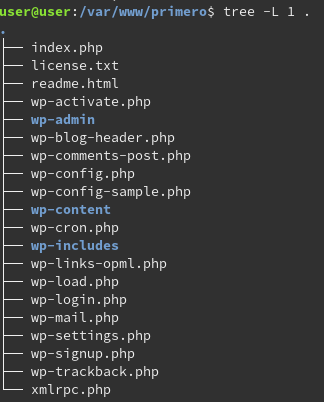
\includegraphics[scale=0.5]{imagenes/img19.png}
\end{minipage}%
\begin{minipage}{0.5\textwidth} % La otra mitad del ancho del texto
    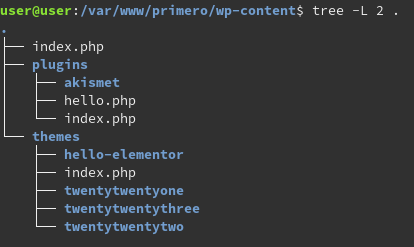
\includegraphics[scale=0.6]{imagenes/img20.png}
\end{minipage}
\end{center}


\subsection{Segunda}
\begin{center}
\begin{minipage}{0.5\textwidth} % La mitad del ancho del texto
    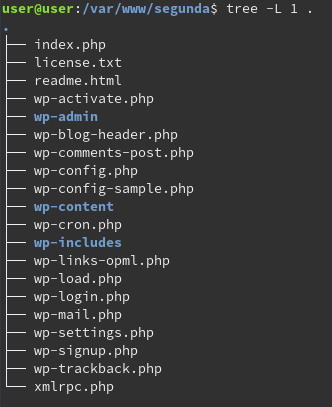
\includegraphics[scale=0.5]{imagenes/img21.png}
\end{minipage}%
\begin{minipage}{0.5\textwidth} % La otra mitad del ancho del texto
    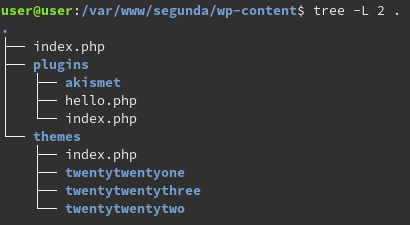
\includegraphics[scale=0.6]{imagenes/img22.png}
\end{minipage}
\end{center}




\newpage
\section{Plantilla WordPress}
\subsubsection{Primera}
\begin{flushleft}
En este punto, ya esta configurado todo lo necesario para que funcionen ambos proyectos, por tanto, vamos a mostrar las plantillas instaladas en wordpress desde el buscador:
\end{flushleft}

\begin{center}
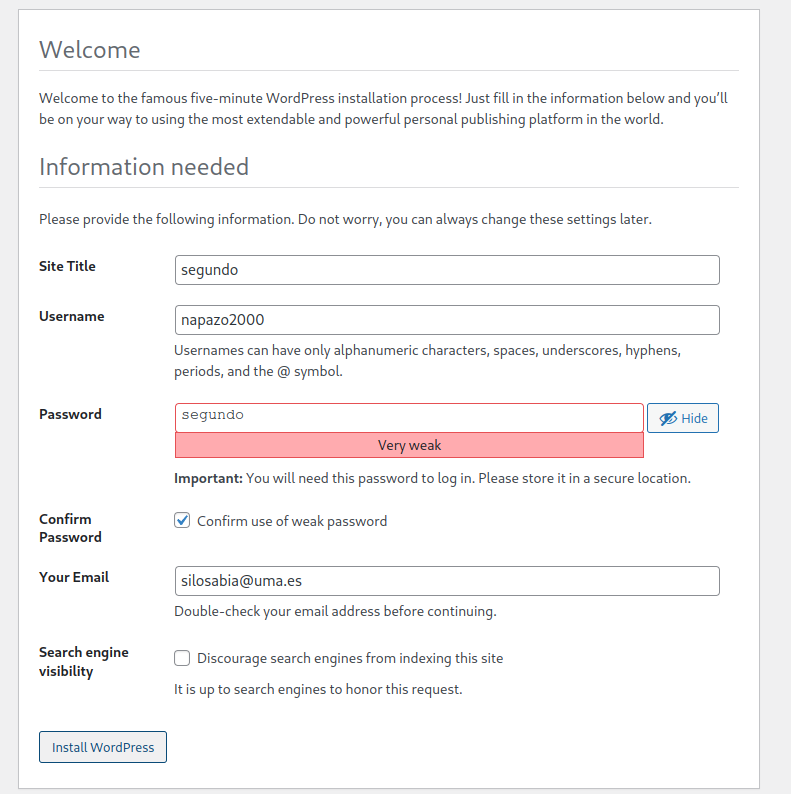
\includegraphics[scale=0.3]{imagenes/im8.png} 
\end{center}

\begin{flushleft}
Una vez que se crea la cuenta, entraremos dentro del dashboard de WordPress para el proyecto
\end{flushleft}

\begin{center}
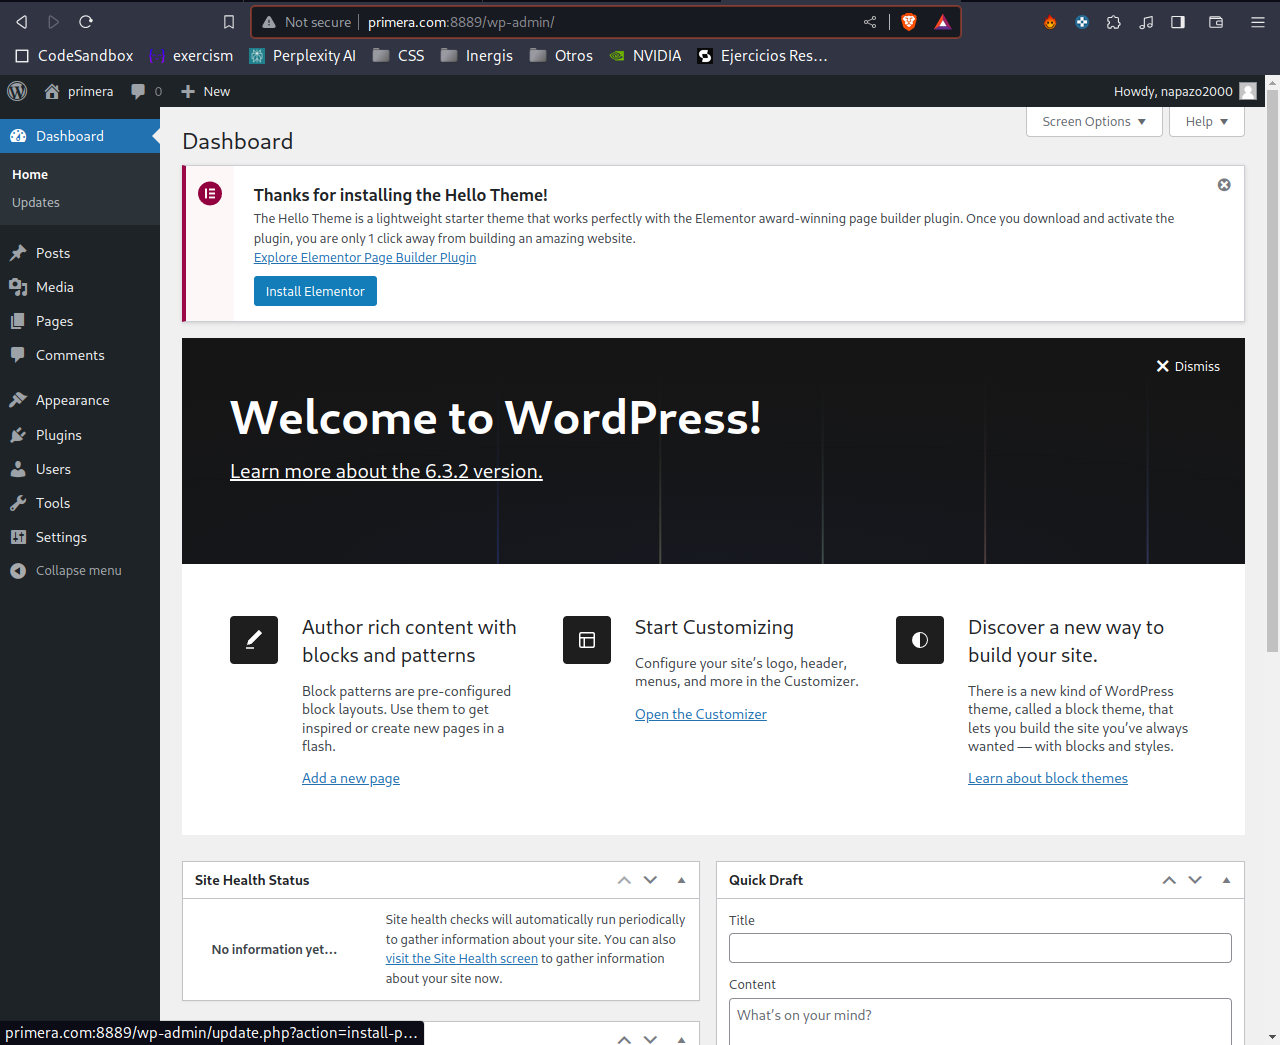
\includegraphics[scale=0.3]{imagenes/img10.png} 
\end{center}

Por último, la vista del usuario:
\begin{center}
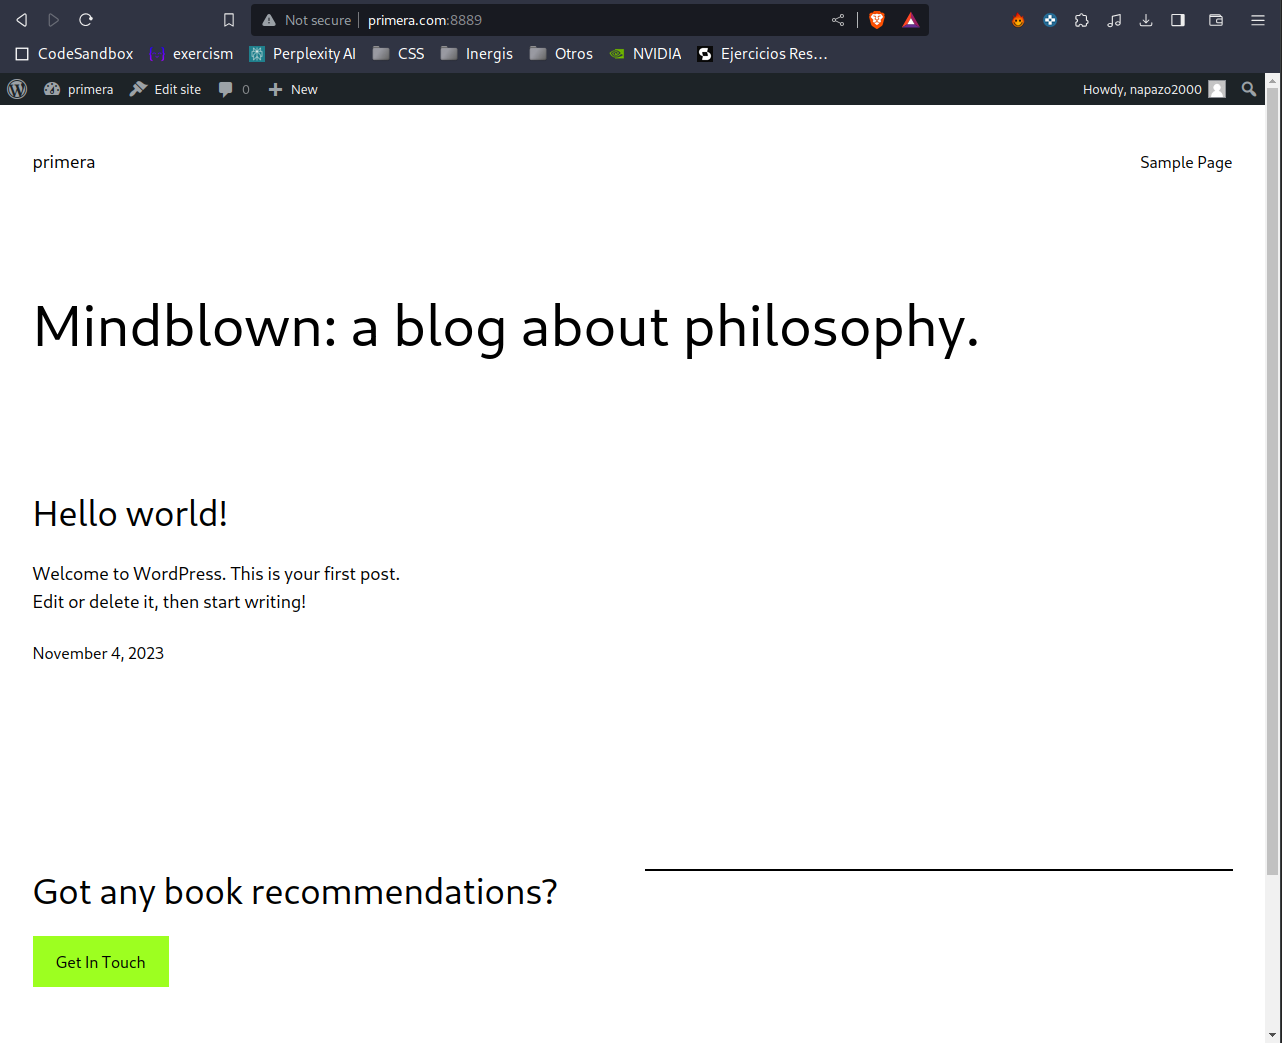
\includegraphics[scale=0.3]{imagenes/img7.png} 
\end{center}


\subsubsection{Segundo}

\begin{center}
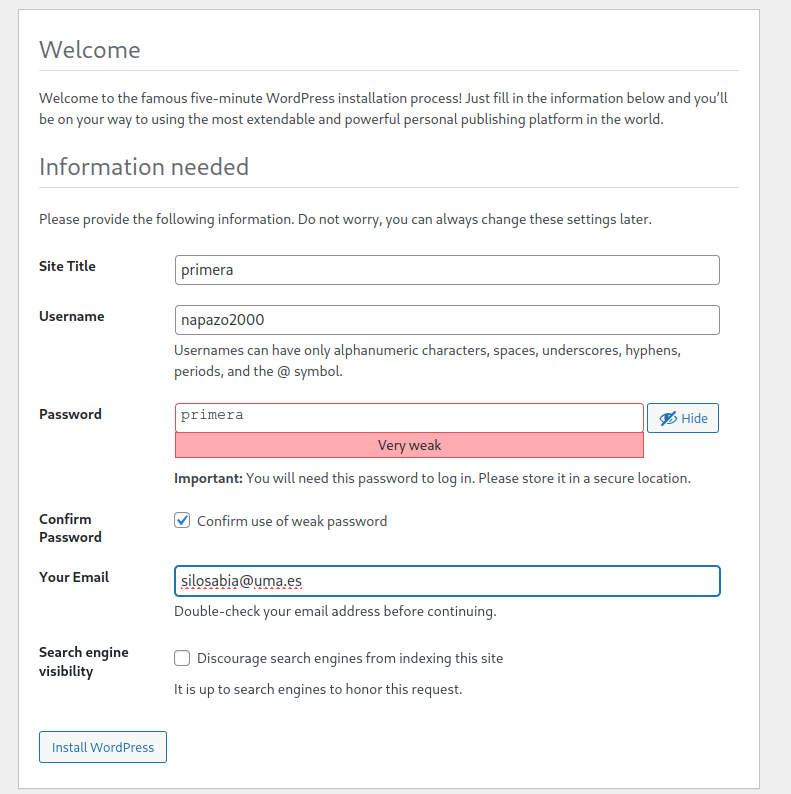
\includegraphics[scale=0.3]{imagenes/img9.png} 
\end{center}

\begin{center}
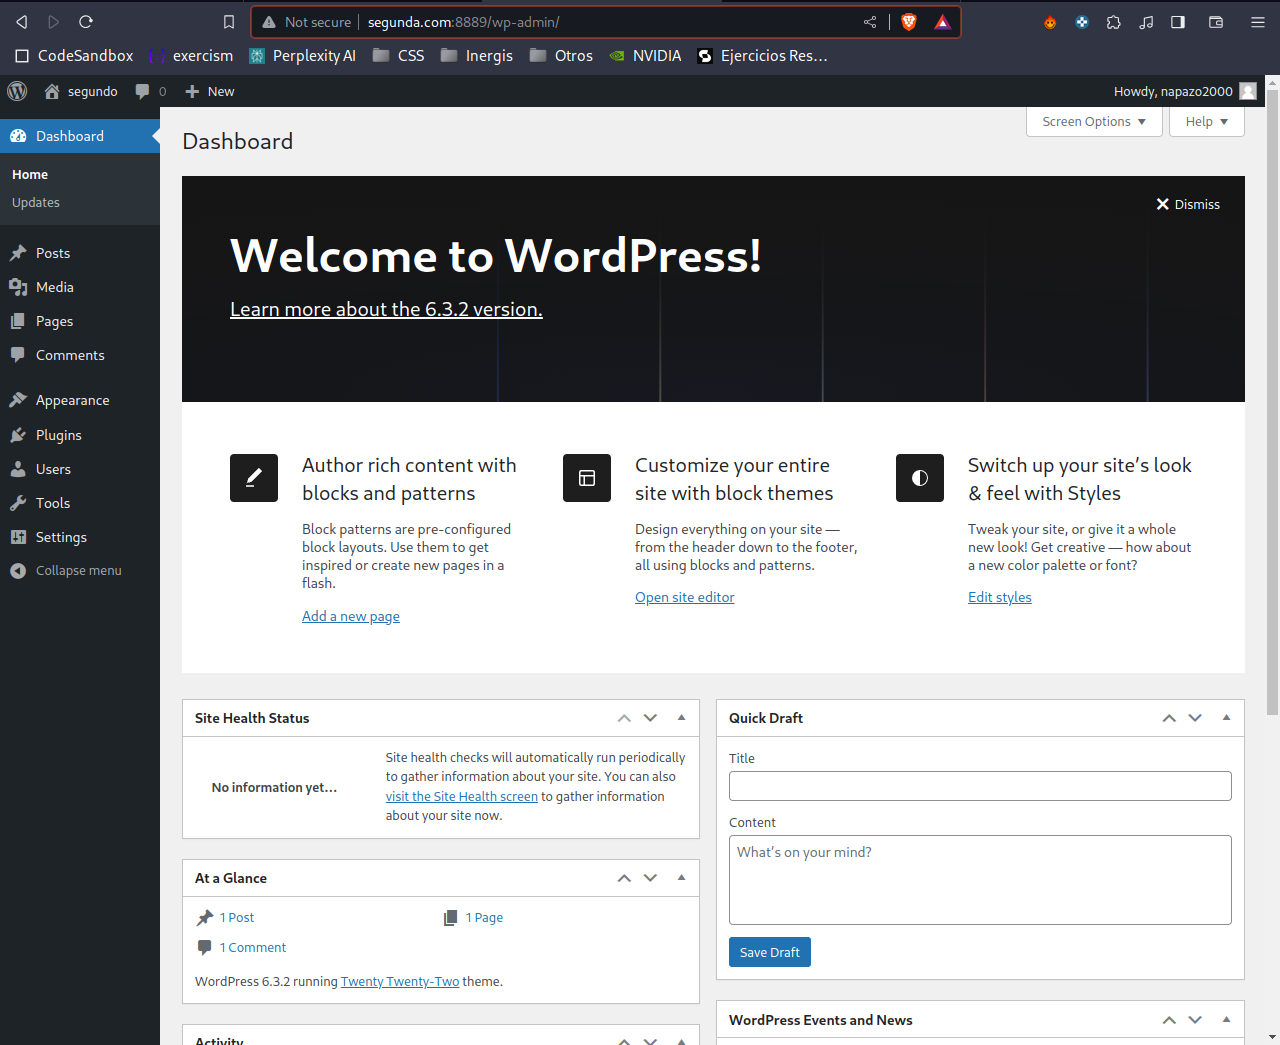
\includegraphics[scale=0.3]{imagenes/img11.png} 
\end{center}


\begin{center}
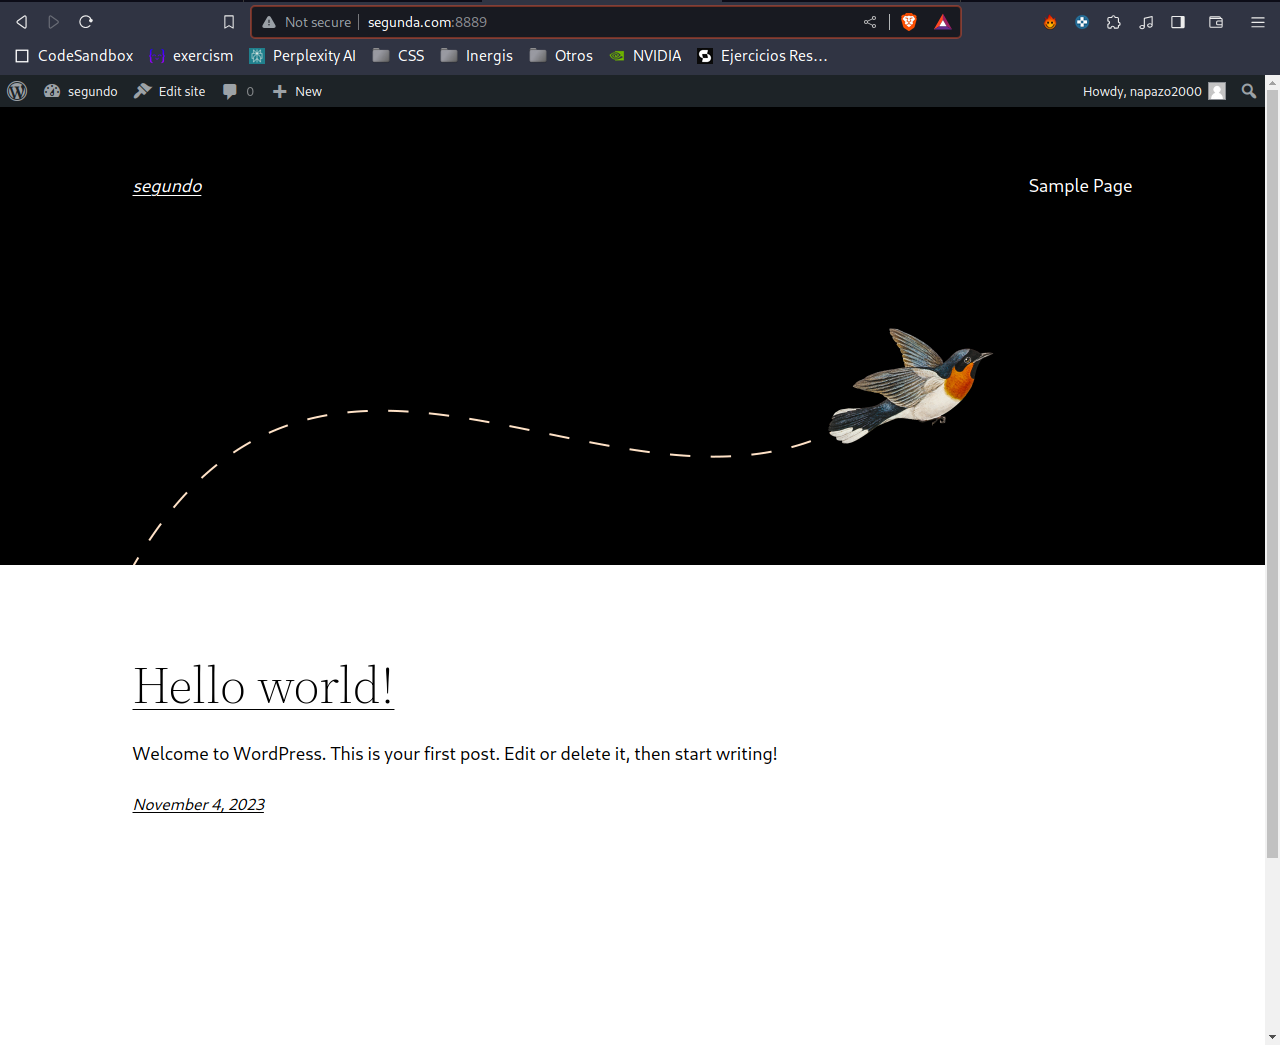
\includegraphics[scale=0.3]{imagenes/img12.png} 
\end{center}

\section{Temas y plugin en WordPress}
Se pueden Modificar y añadir nuevos temas y plugins, tanto dentro de la página de wordpress, como desde terminal, para el primer caso:

\begin{center}
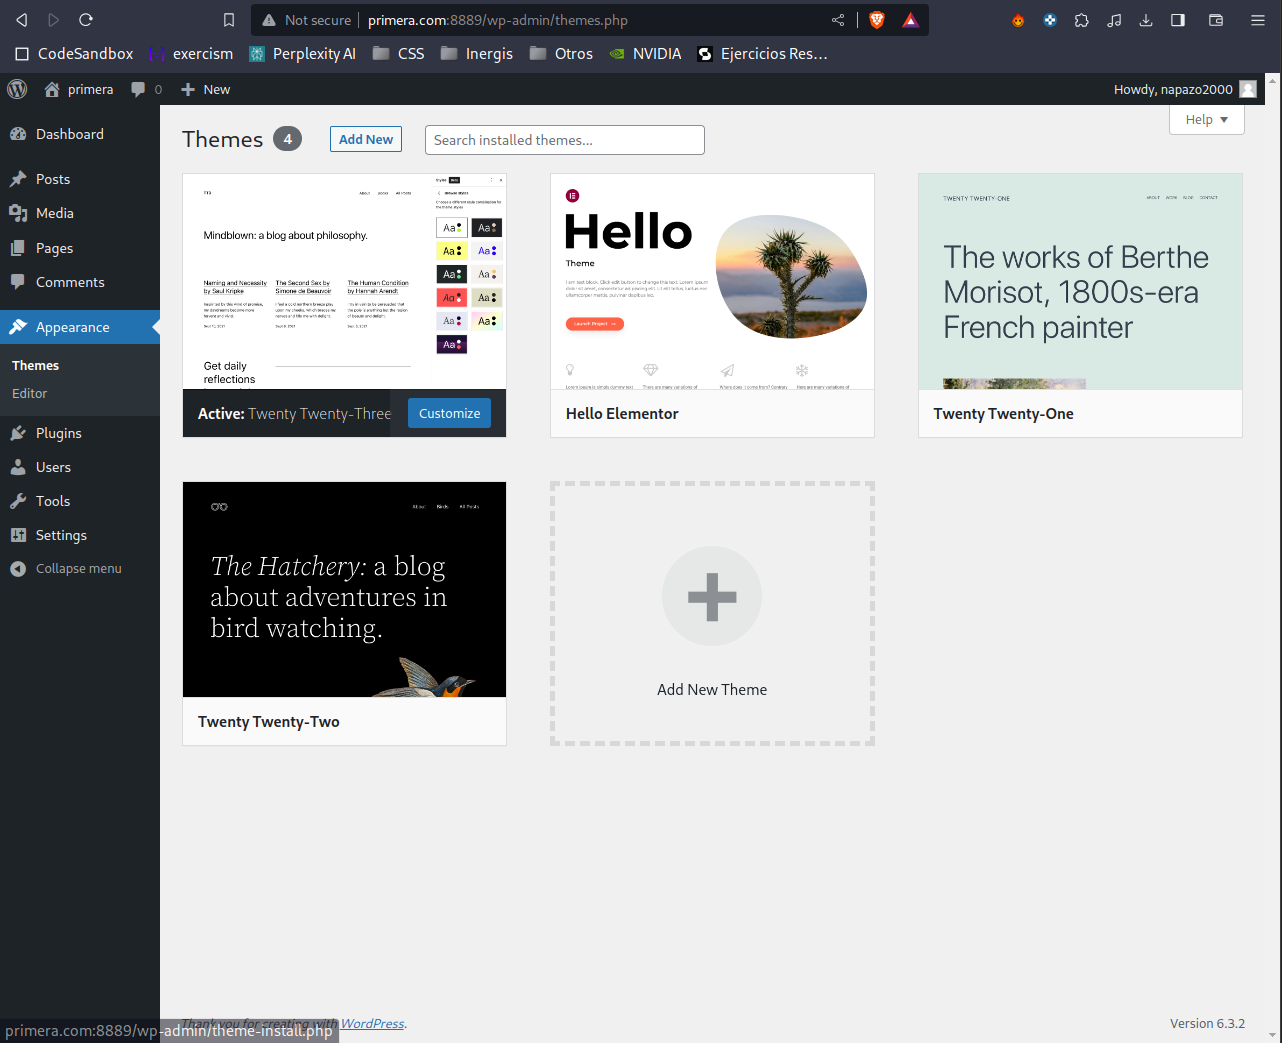
\includegraphics[scale=0.3]{imagenes/img13.png} 
\end{center}

Nos vamos a la página de wordpress.org/themes, y vemos aquellos que hay disponible, para la prueba, vamos a instalar el de PopularFX

\begin{center}
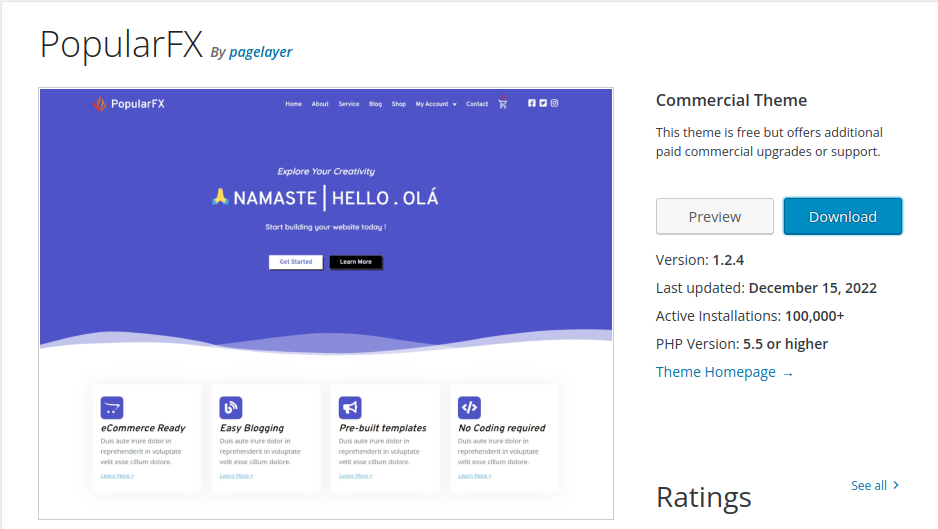
\includegraphics[scale=0.5]{imagenes/img14.png} 
\end{center}

\begin{lstlisting}[frame=single] 
wget https://downloads.wordpress.org/theme/popularfx.1.2.4.zip
unzip popularfx.1.2.4.zip 
sudo mv popularfx /var/www/primero/wp-content/themes/

\end{lstlisting}
\begin{center}
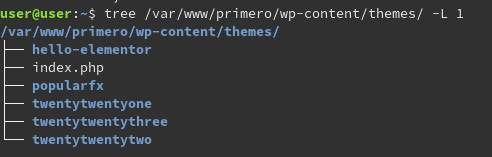
\includegraphics[scale=0.7]{imagenes/img16.png} 
\end{center}

\begin{flushleft}
Ahora, desde la dashboard de Primero, en themes, ya está instalado el nuevo tema:

\end{flushleft}
\begin{center}
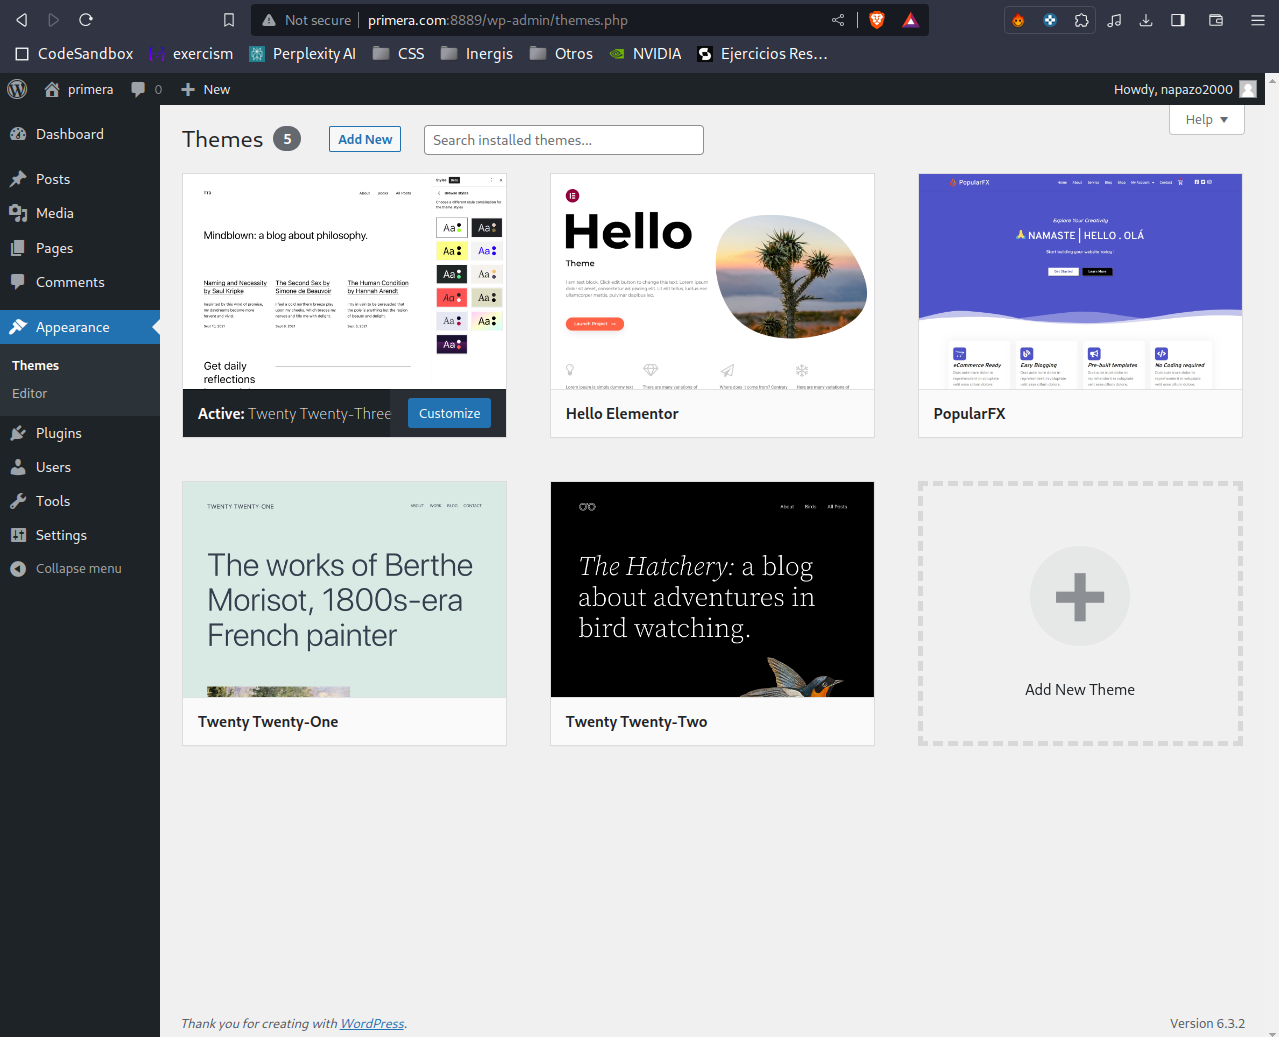
\includegraphics[scale=0.3]{imagenes/img17.png} 
\end{center}

\begin{flushleft}
Aparentemente, este tema, requiere de más configuración que los anteriores, así que, la página por defecto es bastante simple
\end{flushleft}

\begin{center}
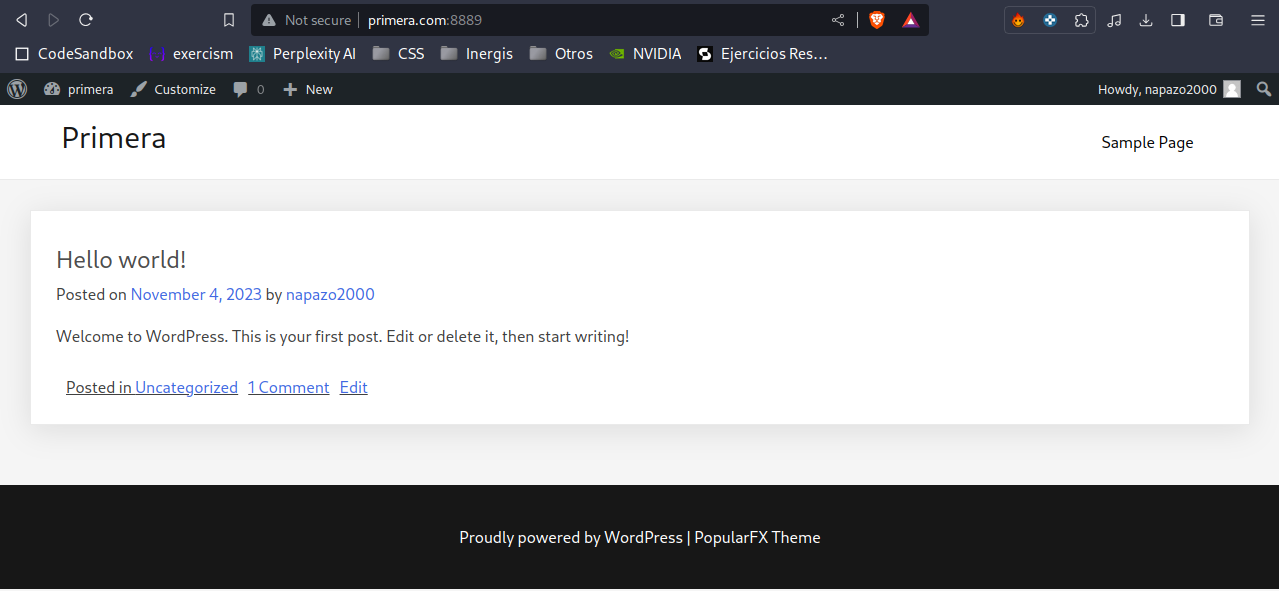
\includegraphics[scale=0.3]{imagenes/img18.png} 
\end{center}

 
 



\end{document}